% QNLPAI 2026 — STUDENT POSTER SESSION ABSTRACT (max 2 pages, Springer LNCS).
% Submit with the draft poster (poster.pdf). Compile on Overleaf (LNCS template) or
% locally: pdflatex abstract && bibtex abstract && pdflatex abstract && pdflatex abstract
%
% SCOPE: deliberately narrowed to TWO objectives (O1 language-conditioned QAOA;
% O2 state-evolution visualization). The risk/IQAE module of QLPC is out of scope here.
% Springer CS proceedings rules honored: LNCS class, splncs04 bib (template default),
% no colour in text/equations, no self-defined environments (only LNCS `credits`).
\documentclass[runningheads]{llncs}
\usepackage[T1]{fontenc}
\usepackage{graphicx}
\usepackage{amsmath,amssymb}
\usepackage[hidelinks]{hyperref}

\begin{document}

\title{Watching Language Steer a Quantum Optimizer: Visualizing the State Evolution of
LLM-Conditioned QAOA for Portfolio Selection}
\titlerunning{Watching Language Steer a Quantum Optimizer}
\author{Pradyot Bathuri\inst{1}}
\authorrunning{P. Bathuri}
\institute{Indiana University, Bloomington, USA \\ \email{pbathuri@iu.edu}}
\maketitle

\begin{abstract}
We ask a narrow question: can a natural-language market view, expressed by a large language model (LLM),
\emph{visibly} steer a quantum optimizer, and can we watch it do so? We encode an LLM view as a tilt on
the expected-return vector of a cardinality-constrained portfolio problem, which deforms the QAOA cost
Hamiltonian, and we snapshot the full statevector after every circuit layer. On exact simulation the
quantum state concentrates on the optimal portfolio, and as linguistic conviction rises the optimum---and
the quantum output that tracks it---migrates across portfolios. This connects two literatures that have
so far stayed apart: LLM-conditioned Black--Litterman allocation (classical) and quantum portfolio
optimization with numerically predicted views (no language, no state visualization).
\keywords{QAOA \and Quantum optimization \and LLM-conditioning \and Quantum finance \and Visualization.}
\end{abstract}

\section{Motivation and Position in the Literature}
Quantum portfolio optimization typically maps asset \emph{selection} to a QUBO solved by
QAOA~\cite{farhi2014qaoa} or VQE, reporting a final bitstring and an approximation ratio. Two limits
motivate us. (i)~The optimizer is opaque: a single scalar hides \emph{how} the state decides, which is
uncomfortable for high-stakes allocation. (ii)~Real allocation is driven by \emph{language}---analyst
theses, filings, news---which has no native port into a QUBO. Recent work touches each side separately.
Lee et al.~\cite{lee2025llmbl} drive Black--Litterman views with an LLM but optimize \emph{classically};
Chen et al.~\cite{chen2023qbl} bring views into a quantum pipeline, yet the views are \emph{numerically
predicted by quantum machine learning} and solved with VQE, with no natural-language input and no view of
the quantum state. We occupy the gap between them, restricting our scope to two tightly-coupled objectives.

\paragraph{Objective 1: Language-conditioned QAOA.}
An LLM reads natural-language views and emits a signed per-asset conviction $v_i\in[-1,1]$; we tilt the
expected returns $\mu\to\mu+s\,v$ (strength $s$), in the spirit of Black--Litterman view-blending
\cite{black1992litterman} but routed into the \emph{quantum} cost Hamiltonian rather than a classical
posterior mean. Holding $B$ of $n$ assets to maximize $\mu^\top x-q\,x^\top\Sigma x$, $x\in\{0,1\}^n$
\cite{markowitz1952}, we minimize $-\mu^\top x+q\,x^\top\Sigma x+P(\sum_i x_i-B)^2$ and substitute
$x_i=(1-z_i)/2$ to obtain a diagonal Ising Hamiltonian $H_C$. Changing the \emph{language} changes $H_C$
and hence the ground state.

\paragraph{Objective 2: Visualizing the state evolution.}
We prepare the uniform superposition and apply, per QAOA layer, $e^{-i\gamma_k H_C}$ then the mixer
$e^{-i\beta_k\sum_j X_j}$ (the diagonal $H_C$ makes the Trotterized evolution exact), training the angles
with restarted COBYLA. We then recompute the statevector incrementally and record $|\psi|^2$ after each
layer, making the optimizer's working process---and the language-induced steering---auditable.

\section{Results and Significance}
All experiments are exact on the statevector simulator with fixed seeds (a well-separated 4-asset
instance, $B{=}2$; reproducible from a single script). \emph{State evolution:} probability migrates from
the uniform superposition ($1/16=0.062$, layers $0.062\to0.25\to0.63$) onto the optimal portfolio at
depth $p{=}2$---P(optimum)$=0.63$, a tenfold concentration over a uniform guess, approximation ratio
$0.92$, with best-sample recovery of the exact optimum; $p{=}4$ reaches $0.75$. \emph{Language steering}
(Fig.~\ref{fig:lang}): a graded LLM bullish view on the two lower-return assets migrates the exact optimum
$\{$A,B$\}\to\{$A,C$\}\to\{$C,D$\}$, and the QAOA modal selection tracks the language-shifted optimum in
all three regimes; concentration is lower under a strong view because the tilt creates genuine near-ties
among portfolios---an honest reflection of ambiguity, not optimizer failure. To our knowledge this is the
first demonstration of a natural-language view visibly deforming the state evolution of a quantum
portfolio optimizer.

\begin{figure}[t]\centering
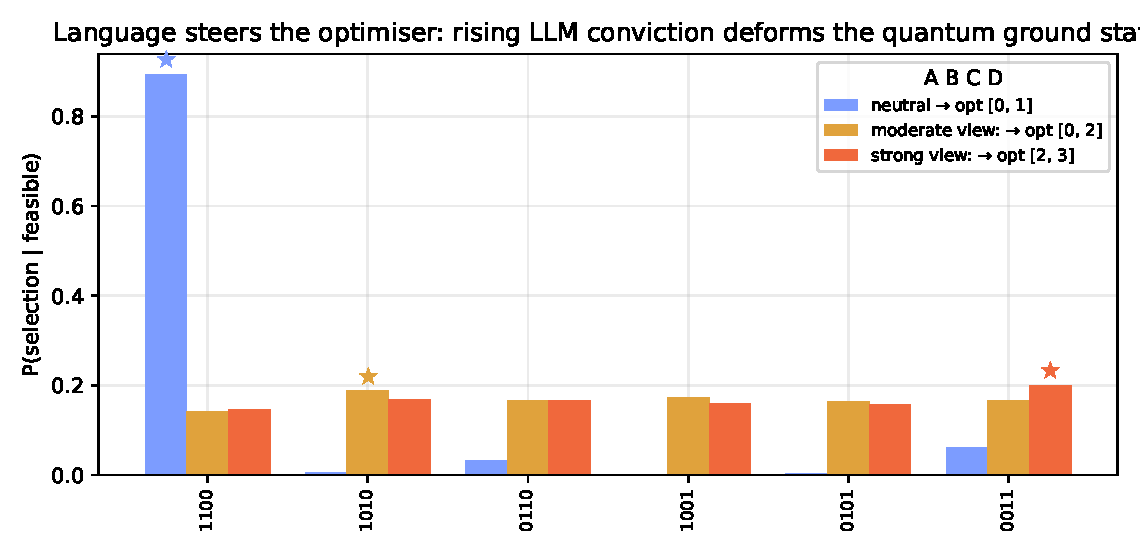
\includegraphics[width=0.84\textwidth]{figures/fig4_language.pdf}
\caption{Language steers the optimizer: as LLM conviction on the lower-return pair rises, the optimum
migrates left-to-right and the QAOA modal selection (star) tracks it across feasible portfolios.}
\label{fig:lang}
\end{figure}

\paragraph{Scope and honesty.}
We deliberately address only the two objectives above; results are on small, well-separated,
exactly-simulated instances. We make no scaling, hardware, or quantum-advantage claim (brute force is our
oracle), and the language tilt is a deliberately simple, interpretable mechanism. The value is a
transparent, reproducible bridge from \emph{language} to a \emph{quantum} optimizer in finance---a
concrete QNLP\,$\times$\,quantum-optimization use case appropriate to a poster that invites discussion.

\begin{credits}
\subsubsection{\ackname}
The author thanks Professor Yuxi Hong for helpful guidance and discussions. Implementation and figure
generation were carried out with the assistance of an AI coding tool; the research questions, the
positioning in the literature, the interpretation of results, and all claims are the author's own, and
every result is reproducible from the released code (\texttt{python -m paper.experiments}, Qiskit~2.x).
\subsubsection{\discintname} The author has no competing interests to declare.
\end{credits}

\bibliographystyle{splncs04}
\bibliography{references}
\end{document}
